\section{ParaReal.jl}

This section describes the general properties of the \julia{ParaReal.jl} package.
It has been designed with the following requirements in mind:
\begin{enumerate}
  \item\label{item:impl:goal:schedule}
    Schedule each stage on a separate process.

    This is a sensible default for the application at hand,
    which is memory bound for typical problem sizes.
    Yet, the scheduling strategy should be modifiable/extendable.
  \item\label{item:impl:goal:variablesize}
    Allow the data transferred be variable in size.

    This is necessary to transmit \ac{LRSIF} of varying rank and, therefore, storage size depending on $n$ (and $k$).
  \item\label{item:impl:goal:notransfer}
    Do not transfer the final solution data back to the calling/managing process.

    For fine resolutions, the storage requirements are immense.
    The overall solution might not fit in memory of a single compute node.
    Therefore, it has to be possible that each stage $n$ saves its local solution along $[t_{n-1},t_n]$ directly to disk,
    without sending it to the calling process first.
\end{enumerate}
On top of that:
\begin{enumerate}[resume]
  \item\label{item:impl:goal:modularity}
    The parareal implementation has to be modular,
    \ie easy to use/adapt for other problems than \ac{LRSIF} formulations of \ac{DRE}.
\end{enumerate}

Requirement \ref{item:impl:goal:schedule} is achieved by the abstract type \julia{Schedule},
whose sole subtype (for now) is \julia{ProcessesSchedule}.
It takes a list of $N$ worker/process ids, each of which will execute one stage.
Future strategies may be implemented by defining new subtype of \julia{Schedule}, \eg
\julia{ThreadsSchedule} using threads on a single process,
\julia{HybridSchedule} which uses both threads and processes, and
\julia{DaggerSchedule} which uses the abstractions provided by \julia{Dagger.jl}.\footnote{\url{https://github.com/JuliaParallel/Dagger.jl}}

Requirement \ref{item:impl:goal:variablesize} is trivial to fulfill using Julia's \julia{RemoteChannel} data type.
Requirement \ref{item:impl:goal:modularity} imposes a non-specific naming scheme for
user interface functions and the name of the unknown,
as to not clash with the standard nomenclatures of other disciplines.\footnote{%
  For example,
  many parareal papers use $U$ to name the unknown,
  many matrix \ac{ODE} papers use $X$,
  and the widely-used \julia{DifferentialEquations.jl} package~\cite{DifferentialEquations} uses $u$.
}
The next section will describe the user interface of the \julia{ParaReal.jl} package,
and how to cope with problem~\ref{item:impl:goal:notransfer}.

\subsection{User Interface}

In applications one is usually interested in a high temporal resolution,
while the parareal method is only used to obtain \enquote{fast} convergence.
Therefore, the \julia{ParaReal.jl} package distinguishes between a local solution along $[t_{n-1}, t_n]$ and the final value of which,
\begin{align*}
  F(U_{n-1}^k) &= \julia{value(fsolve(prob))} \\
  G(U_{n-1}^k) &= \julia{value(csolve(prob))}
\end{align*}
where \julia{prob} is an instance of the global \ac{IVP}~\eqref{eq:IVP}
restricted to the local time slice~$[t_{n-1}, t_n]$ and initial value~$U_{n-1}^k$.
The actual solver functions \julia{csolve} (\enquote{coarse}) and \julia{fsolve} (\enquote{fine})
are provided as arguments to \julia{ParaReal.Algorithm()}.
In order to support custom \ac{IVP} types,
a user has to defined methods for \julia{initial\_value()} to extract the global initial value $U_0$,
and \julia{remake\_prob()} to adjust the global problem for the local time slice and initial value.
For more details, refer to the documentation of the respective functions available from within Julia.

In order to support new solution types,
a custom implementation of the parareal update formula~\eqref{eq:pr:method} may be needed.
This can be specified as an optional third argument to \julia{ParaReal.Algorithm}.
The default is \julia{ParaReal.default\_update!()},
whose implementation is given in~\autoref{lst:impl:default_update!}.
Adding methods to \julia{default\_update!()} is not recommended.
Any custom implementation of the parareal update formula must follow the interface of \julia{default\_update!()}.

\def\sk{\textsuperscript{k}}
\def\skmi{\textsuperscript{k-1}}
\begin{lstlisting}[%
  float=t,
  label={lst:impl:default_update!},
  caption={Default implementations of the parareal update formula},
  escapechar=\%,
  breaklines=true,
]
function default_update!(_, G%\sk%, F%\skmi%, G%\skmi%)
    G%\sk% + F%\skmi% + (-G%\skmi%) # out-of-place
end

function default_update!(U%\sk%::Array, G%\sk%, F%\skmi%, G%\skmi%)
    @. U%\sk% = G%\sk% + F%\skmi% - G%\skmi% # in-place
end
\end{lstlisting}

The remainder of this section is devoted to a complete example of a user-defined problem type ($N=3$, $K=2$).
The problem type will be a mere placeholder that forwards its initial value,
while the solver functions will count the applications of $F$ and $G$ a particular solution is composed of.
Start by launching some worker processes and loading the necessary packages:
\lstinputlisting[%
  caption={User-defined problem type for \julia{ParaReal.jl}},
  label={lst:impl:parareal_counting},
  lastline=5,
]{code/parareal_counting.jl}
Next, define the problem type and ensure that definition is available on all processes.
The only requirement to the problem type is to have a \julia{tspan} field.\footnote{%
  Alternatively, it must support \julia{getproperty(prob, :tspan)}.
}
In the context of \ac{ODE}, this should not clash with any other notation.
\addtocounter{lstnumber}{1} %FIXME
\lstinputlisting[nolol, firstnumber=last, linerange=problem-end]{code/parareal_counting.jl}
The solution type will hold counters of the applications of $F$ and $G$:
\lstinputlisting[nolol, firstnumber=last, linerange=solution-end]{code/parareal_counting.jl}
Define the solver functions and problem instance and execute the parareal pipeline.
The solver functions are defined as closures,
such that they can be serialized and transferred to the worker processes.
Note that this code is only executed on the managing process:
\lstinputlisting[nolol, firstnumber=last, linerange=solve-end]{code/parareal_counting.jl}
Lastly, extracting the final values $U_1^1$, $U_2^2$, and $U_3^2$ via
\lstinputlisting[nolol, firstnumber=last, linerange=result-end]{code/parareal_counting.jl}
yields:
\begin{align*}
  &\julia{Counters(1,0)}, \text{ since} &
  U_1^1 &= F(U_0) \\
  &\julia{Counters(2,0)}, \text{ since} &
  U_2^2 &= F(F(U_0)) \\
  &\julia{Counters(3+2+2,2+4+4)}, \text{ since} &
  U_3^2 &= G(F(F(U_0))) + F(U_2^1) - G(U_2^1) \\
  && U_2^1 &= G(F(U_0)) + F(G(U_0)) - G(G(U_0))
\end{align*}

The full trajectory of the fine solver may be extracted using \julia{ParaReal.solution()}.
However, solution and value are identical in the example above,
\cf line~\ref{line:impl:parareal_counting:value}.
\autoref{lst:impl:store} shows the recommended pattern of
storing the fine solutions directly from the worker processes
via \julia{ParaReal.fetch\_from\_owner()}.

\begin{lstlisting}[%
  float=tpb, % TODO: ensure this doesn't disrupt the inline code snippets
  caption={%
    [Store fine parareal solutions directly from the worker processes]
    Store fine parareal solutions directly from the worker processes.
    This works well as a blueprint for \julia{DrWatson.\_wsave(dir, sol)} \cite{DrWatson}.
  },
  label={lst:impl:store},
]
using ParaReal: fetch_from_owner

# Assume solution to be given:
sol::ParaReal.Solution

# Ensure output directory exists:
mkpath(dir)

@sync for sref in sol.stages
    @async fetch_from_owner(sref) do s::ParaReal.Stage
        sol = ParaReal.solution(s)
        tmin, tmax = extrema(sol.t)
        fname = joinpath(dir, "t=$tmin:$tmax.h5")
        # Write `sol` to `fname`, e.g. via
        DrWatson.wsave(fname, sol)
    end
end
\end{lstlisting}

\subsection{JIT Compilation and Warm-Up}

Julia is a \ac{JIT} compiled language~\cite{Julia},
which means that code is compiled just before it is first executed,
unless it has already been compiled.
Therefore, unless the code has been compiled \ac{AOT},
only the second execution of code is fast.
This effect is called \emph{warm-up}.
As mentioned in~\autoref{sec:pr}, computing the coarse solutions
$G(U_n^*)$ is essentially a sequential operation over all $n$.
The computations of $F(U^*_n)$ can only be parallelized after such a global coarse solve.
Therefore, it is critical that the individual coarse solutions are available as fast as possible.

\todo[inline]{Describe notion of \enquote{ramp-up delay}?}

\begin{figure}[tb]
  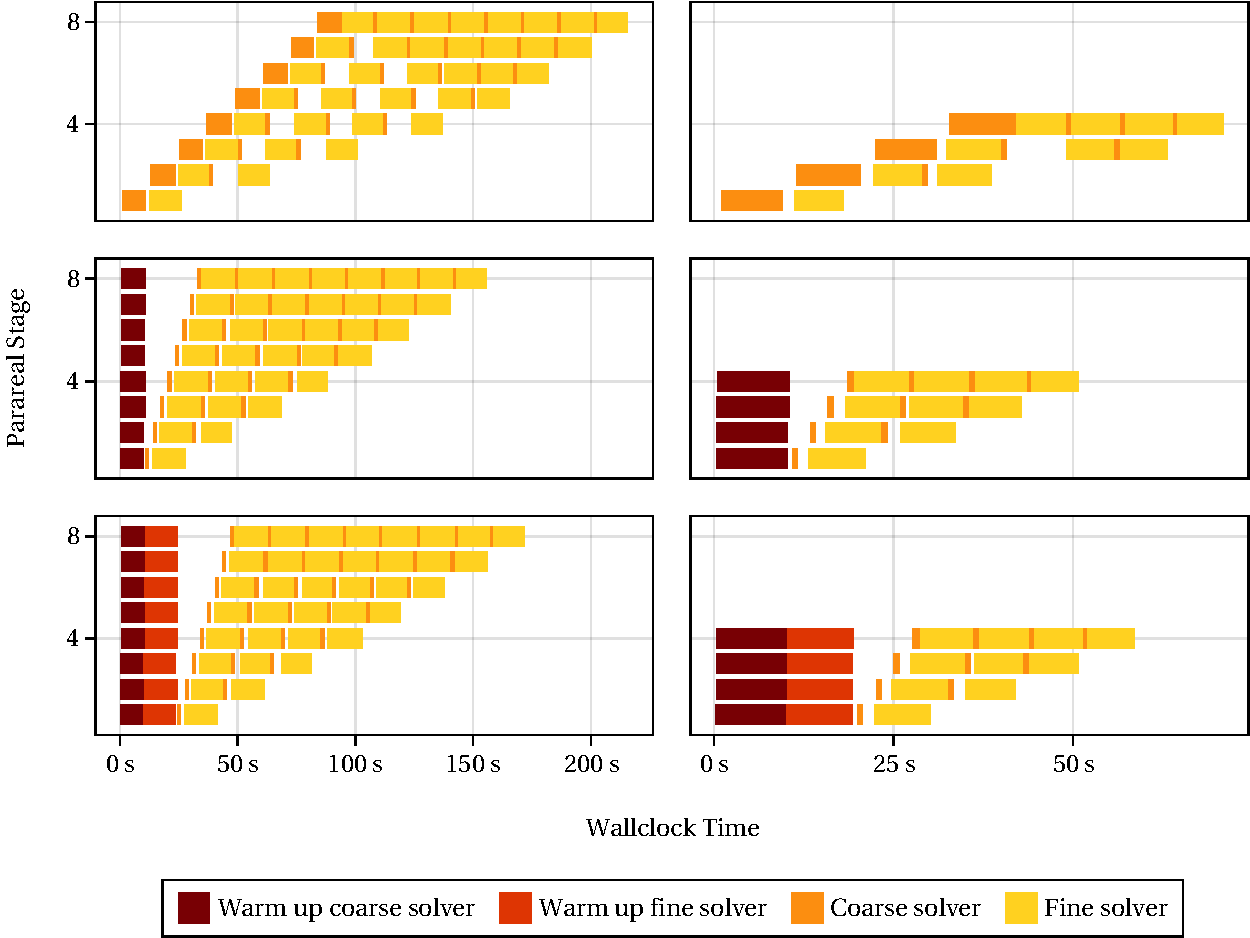
\includegraphics[width=\textwidth]{figures/fig_impl_warmup2.pdf}
  \caption[Timeline diagrams comparing the effect of JIT compiler warm-up.]{%
    Timeline diagrams comparing the effect of \acs{JIT} compiler warm-up.
    Left: $N=8$ processes running on two compute nodes,
    right: $N=4$ processes running on a laptop.
    Top: no warm-up,
    middle: warming up coarse solver \julia{csolve} ($G$),
    bottom: warming up coarse and fine solver \julia{fsolve} ($F$).
  }
  \label{fig:impl:warmup}
\end{figure}

\begin{table}[tb]
  \caption{Ramp-up delay}
\end{table}

\paragraph{Sequential \ac{JIT} compilation}

Without any precautions,
\ac{JIT} compilation of $G$ happens sequentially,
as computing $G(U_n^k)$ is essentially sequential.
This effect is especially severe if the executors of different parareal iterations $(n,k)$ do not share the results of code compilation.
These executors may be processes, threads~(pthreads), or tasks~(green threads).
As of the writing of this thesis,
there is a one-to-one mapping between processes and stages $n$,
which means the compilation happens exactly once per stage $n$ and is reused between refinements $k$.\footnote{%
  As of the writing of this thesis, Julia does not reuse code compiled between processes.
}
This is visible in the first row of \autoref{fig:impl:warmup}
by the first occurrences of $G$ for each stage $n$,
which marks the computation of $G(U_n^0)$,
whose execution time includes compilation time.

\paragraph{Parallel \acs{AOT} compilation}

Since \julia{ParaReal.jl} is independent of $F$ and $G$ as well as the actual data type of the underlying \ac{IVP},
full \ac{AOT} compilation is difficult, and has to be done by users of the package.
A more naive approach is to manually warm up critical parts of the code by executing them before they are actually needed.
In the context of \julia{ParaReal.jl},
doing so allows to perform the compilation in parallel,
which significantly decreases the time to compute all coarse solutions $G(U_n^*)$.
This is visible in the middle and bottom rows of \autoref{fig:impl:warmup}.
$F$ and $G$ have a lot of code in common,\footnote{%
  For example, the Lyapunov solvers will be called with arguments having the exact same types,
  \ie they will call the same method internally.
  Unless that method has been inlined, the results of its compilation will be reused.
}
such that warming up both shows a much smaller improvement compared to just warming up the coarse solver $G$.

\paragraph{Precompilation}

Besides reducing the delay of executing $F$ and $G$,
it is also important to reduce the delay of any code from \julia{ParaReal.jl} that doesn't depend on them.
The package is merely responsible for orchestrating the execution of the parareal iterations $(n,k)$.
Therefore, the delay of the first execution of \julia{ParaReal.jl} code is dominated by type inference.\footnote{%
  At least it likely is. Taking measurements is highly non-trivial and out of the scope of this thesis.
  For more details see: \url{https://julialang.org/blog/2020/08/invalidations/}
}
The time spent on type inference can be minimized by precompilation,
which happens when the package is first loaded,
and whose results are cached and reused when the package is loaded again.
Exploiting this is highly non-trivial and out of the scope of this thesis.\footnote{\url{https://julialang.org/blog/2021/01/precompile_tutorial/}}

\todo[inline]{%
How to cite these webpages properly?
Should I do anything about the speculation in the paragraph, or the exposure of which in the footnote?
}

\subsection{Lack of Asynchronous Data Transfer}

A common strategy to improve CPU utilization is to perform data transfers between processes asynchronously.
Julia offers the \julia{RemoteChannel} data structure for this purpose.
As of the writing of this thesis,
the \julia{RemoteChannel} is not thread-safe.\footnote{\url{https://github.com/JuliaLang/julia/issues/37706}}
More specifically, it must be used from thread~1 of each process.
This means that in order to asynchronously send the interface~values~$U_n^{k+1}$ from stage $n$ to the next,
one would have to move the calls to~$F$ and~$G$ off of thread~1.
The reason is that many implementations of $F$ and $G$ don't have an implicit (cooperative) yield point to Julia's runtime,
such that no task can run asynchronously on thread~1 next to the task executing~$F$ and~$G$.
This is particularly true for code that doesn't require~\ac{IO},
\eg for many methods from Julia's \julia{LinearAlgebra} standard library,
which internally call \code{LAPACK}.

\todo{Mention that Julia runs single-threaded as to not oversaturate machine? BLAS/LAPACK launch their own threads.}
The solution described in the previous paragraph is not yet implemented,
\ie all data transfers are synchronous.
This causes gaps visible in \autoref{fig:impl:warmup} after $G$ and before $F$,
whose ends roughly align with the beginnings of calls to $G$ on the next stage.

Another effect is that the iterations $(n,k)$ for which $n+k \geq N$ do not show this gap.
The reason is twofold.
The last stage $N$ doesn't need to send any data, therefore has no \ac{JIT} warm-up delay for the first iteration $k=0$ and no gap in the diagram.
This causes the next refinement $k=1$ of the previous stage $N-1$ to have a noticeably smaller gap,
since its transmission code has already been compiled.
This effect propagates back-to-front through the still running pipeline stages.

The exact size of the gap between the computations of $G(U_{n-1}^k)$ and $F(U_{n-1}^k)$ of stage $n$ is determined by
\begin{enumerate}
  \item\label{item:impl:gapsize:1}
    the execution time of the transfer of $U_n^k$ to stage $n+1$, and
  \item\label{item:impl:gapsize:2}
    the overhead included in the computation of $G(U_n^{k-1})$,
    \ie the previous iterate $k-1$ on the next stage $n+1$.
\end{enumerate}
For $k=0$, \ref{item:impl:gapsize:2} is zero.
For $k=1$ and no warm-up, \ref{item:impl:gapsize:2} includes compilation time and dominates \ref{item:impl:gapsize:1},
which shadows the effect described in the previous paragraph for the first row of \autoref{fig:impl:warmup}.
For $k\geq 2$, \ref{item:impl:gapsize:2} is essentially zero.\footnote{%
  If due to user code the data types of $U_n^*$ changes, recompilation might be necessary.
}

\subsection{Advanced Scheduling Strategies}

\begin{itemize}
  \item
    Early stages $n=0,1,2$ become idle even before later stages receive their first $U^0_n$.
    Maybe they could be reused: measure runtime of $F$ and $G$ to compute optimum number $N$ for given number of processors.
    Alternatively, one could adjust the local time slices, \cf \url{https://gitlab.mpi-magdeburg.mpg.de/jschulze/ParaReal.jl/-/issues/2}
  \item
    If $X$ trajectories shall not be saved, solving the \ac{DRE} isn't that memory heavy.
    Creating a connection between workers in a cluster shouldn't be that expensive (they are initialized lazily, but cost should pay off).
    It might be worth it to send $U^{k+1}_n$ as well as $G(U^k_n)$ and $F(U^k_n)$ over the network in order to recycle processors.
    However, this requires a lazy DAG scheduling like \texttt{DAGGER.jl}.
  \item
    \cite[493]{Nielsen2018} relevant?
  \item
    Distributed processes vs local threads vs GPU?
\end{itemize}

